\chapter{INTRODUCTION}
\section{What's {\iqist}?}

The Interacting Quantum Impurity Solver Toolkit (dubbed {\iqist}) is an open source software package aiming to provide a full, reliable, flexible, and powerful tool chain for various quantum impurity models. It contains a few continuous-time quantum Monte Carlo impurity solvers (hybridization expansion version), a Hirsch-Fye quantum Monte Carlo impurity solver, and numerous prep-processed and post-processed tools. The {\iqist} is an all-in-one package. With it you can solve quantum impurity models and anaylyze the calculated results easily and efficiently.

\section{Motivation}

%% DMFT
Dynamical mean-field theory (DMFT)~\cite{RevModPhys.68.13} and its cluster extensions~\cite{RevModPhys.77.1027,RevModPhys.78.865} play a very important role in contemporary studies of correlated electron systems. The broad applications of this technique range from the study of Mott transitions~\cite{PhysRevB.54.8452,PhysRevLett.101.186403}, unconventional superconductivity in Cu- and Fe-based superconductors~\cite{PhysRevLett.96.047005,Yin2011,PhysRevLett.106.047004,Wang13,PhysRevLett.110.216405,PhysRevB.88.245110}, and non-Fermi liquid behaviors~\cite{PhysRevLett.102.206407,PhysRevLett.108.216401,PhysRevLett.110.086401}, to the investigation of anomalous transport properties of transition metal oxides~\cite{RevModPhys.70.1039}. For many of these applications, DMFT is the currently most powerful and reliable (sometimes the only) technique available and has in many cases produced new physical insights. Furthermore, the combination of \emph{ab initio} calculation method (such as density function theory) with DMFT~\cite{RevModPhys.78.865} allows to compute the subtle electronic properties of realistic correlated materials, including partially filled $3d$- and $4d$-electron transition metal oxides, where lattice, spin and orbital degrees of freedom all coupled~\cite{RevModPhys.70.1039}.

%% impurity solvers
The key idea of DMFT is to map the original correlated lattice model into a quantum impurity model whose mean-field bath is determined self-consistently~\cite{RevModPhys.68.13,RevModPhys.77.1027,RevModPhys.78.865}. Thus, the central task of a DMFT simulation becomes the numerical solution of the quantum impurity problem. During the past several decades, many methods have been tested as impurity solvers, including the exact diagonalization (ED)~\cite{PhysRevLett.72.1545}, equation of motion (EOM)~\cite{PhysRevB.50.7295}, Hubbard-I approximation (HIA)~\cite{PhysRevB.39.6962}, iterative perturbation theory (IPT)~\cite{PhysRevB.45.6479}, non-crossing approximation (NCA)~\cite{Grewe1983,Kuramoto1983,RevModPhys.59.845}, fluctuation-exchange approximation (FLEX)~\cite{Bickers1989206,PhysRevB.43.8044}, and quantum Monte Carlo (QMC)~\cite{PhysRevLett.56.2521,PhysRevLett.69.168}. Among the methods listed above, the QMC method has several very important advantages, which makes it so far the most flexible and widely used impurity solver. First, it is based on the imaginary time action, in which the infinite bath has been integrated out. Second, it can treat arbitrary couplings, and can thus be applied to all kinds of phases including the metallic phase, insulating state, and phases with spontaneous symmetry breaking. Third, the QMC method is numerically exact with a ''controlled" numerical error. In other words, by increasing the computational effort the numerical error of the QMC simulation can be systematically reduced. For these reasons, the QMC algorithm is considered as the method of choice for many applications.

%% CTQMC impurity solvers
Several QMC impurity solvers have been developed in the past three decades. An important innovation was the Hirsch-Fye QMC (HF-QMC) impurity solver~\cite{PhysRevLett.56.2521,PhysRevLett.69.168}, in which the time axis is divided into small time steps and the interaction term in the Hamiltonian is decoupled on each time step by means of a discrete Hubbard-Stratonovich auxiliary field. HF-QMC has been widely used in the early studies of DMFT~\cite{RevModPhys.68.13,RevModPhys.77.1027, RevModPhys.78.865}, but is limited by the discretization on the time axis and also by the form of the electronic interactions (usually only density-density interactions can be treated). Recently, a new class of more powerful and versatile QMC impurity solvers, continuous-time quantum Monte Carlo (CT-QMC) algorithms, have been invented~\cite{PhysRevB.72.035122,Gull2008,PhysRevB.74.155107,PhysRevB.75.155113,PhysRevLett.97.076405,RevModPhys.83.349}. In the CT-QMC impurity solvers, the partition function of the quantum impurity problem is diagrammatically expanded, and then the diagrammatic expansion series is evaluated by stochastic Monte Carlo sampling. The continuous-time nature of the algorithm means that operators can be placed at any arbitrary position on the imaginary time interval, so that time discretization errors can be completely avoided. Depending on how the diagrammatic expansion is performed, the CT-QMC approach can be further divided into interaction expansion (or weak coupling) CT-QMC (CT-INT)~\cite{PhysRevB.72.035122}, auxiliary field CT-QMC (CT-AUX)~\cite{Gull2008}, and hybridization expansion (or strong coupling) CT-QMC (CT-HYB)~\cite{PhysRevLett.97.076405,PhysRevB.74.155107,PhysRevB.75.155113}.

%% CT-HYB
At present, the CT-HYB is the most popular and powerful impurity solver, since it can be used to solve multi-orbital impurity model with general interactions at low temperature~\cite{RevModPhys.83.349}. In single-site DMFT calculations, the computational efficiency of CT-HYB is much higher than that of CT-INT and HF-QMC, especially when the interactions are  strong. However, in order to solve more complicated quantum impurity models (for example, five-band or seven-band impurity model with general interactions and spin-orbital coupling) efficiently, further improvements of the CT-HYB impurity solvers are needed. In recent years many tricks and algorithms have been developed to increase the efficiency and accuracy of original CT-HYB impurity solver, such as the truncation approximation~\cite{PhysRevB.75.155113}, Krylov subspace iteration~\cite{PhysRevB.80.235117}, orthogonal polynomial representation~\cite{PhysRevB.84.075145,PhysRevB.85.205106}, PS quantum number~\cite{PhysRevB.86.155158}, lazy trace evaluation and skip listing methods~\cite{arXiv:1403.7214}, and matrix product state implementation~\cite{1742-5468-2014-6-P06012}. As the state-of-the-art CT-HYB impurity solvers become more sophisticated and specialized, it is not easy anymore to master all their facets and build ones implementations from scratch. Hence, we believe that it is a good time to provide a CT-HYB software package for the DMFT community such that researchers can focus more on the physical questions, instead of spending much time on (re-)implementing efficient codes. In fact, there are some valuable efforts in this direction, such as TRIQS~\cite{triqs}, ALPS~\cite{1742-5468-2011-05-P05001}, w2dynamics~\cite{w2dynamics}, Haule's code~\cite{haule}, etc. However, a flexible, extensible, and highly efficient CT-HYB impurity solver is still lacking. The purpose of this reference manual is to present our solution -- the open source software package {\iqist} -- which contains several well-implemented and thoroughly tested modern CT-HYB impurity solvers, and the corresponding pre- and post-processing tools.

\section{Software architecture}
\begin{figure}[ht]
\centering
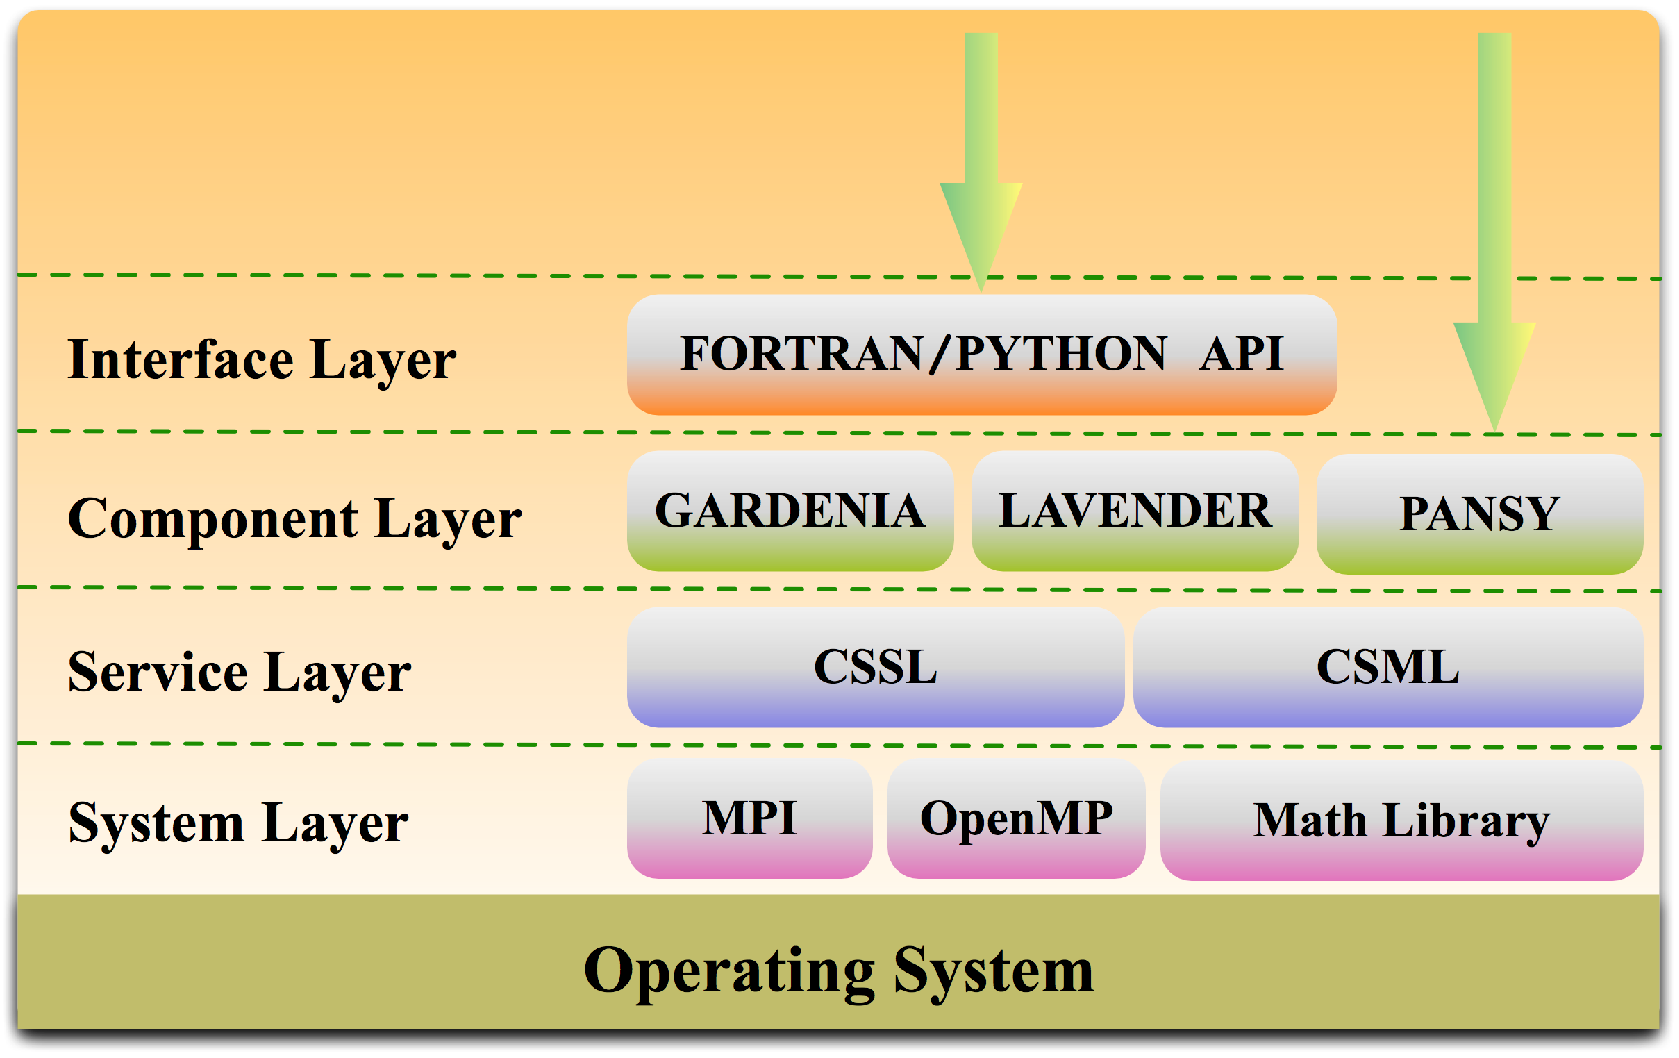
\includegraphics[width=1.0\textwidth]{figure/iqist_structure.pdf}
\caption[The hierarchical structure of the {\iqist} software package]{The hierarchical structure of the {\iqist} software package. Note that in the component layer, not all of the components are listed due to space limitations. See the main text for detailed explanations. \label{fig:framework}}
\end{figure}

\begin{figure}[ht]
\centering
\scalebox{0.95}{\begin{tikzpicture}[mindmap, concept color=black, text=white]
    \node[concept, minimum size=2.6cm] {$i$QIST's\\ Components}
        child[concept color=blue, grow=000, minimum size=2.4cm] {node[concept]{DAISY}}
        child[concept color=olive, grow=045, minimum size=2.4cm] {node[concept]{JASMINE}}
        child[concept color=lime!80!black, grow=315, minimum size=2.4cm] {node[concept]{HIBISCUS}}
        child[concept color=red, grow=180, minimum size=2.4cm] {node[concept]{AZALEA}
            child[concept, grow=120, minimum size=2.2cm] {node[concept]{GARDENIA}}
            child[concept, grow=240, minimum size=2.2cm] {node[concept]{NARCISSUS}}}
        child[concept color=orange, grow=225, minimum size=2.4cm] {node[concept]{BEGONIA}
            child[concept, grow=225, minimum size=2.2cm] {node[concept]{LAVENDER}}}
        child[concept color=magenta, grow=135,minimum size=2.4cm] {node[concept]{PANSY}
            child[concept, grow=135, minimum size=2.2cm] {node[concept]{MAN\-JUSHAKA}}};
\end{tikzpicture}}
\caption[Schematic picture for the {\iqist}'s components]{Schematic picture for the {\iqist}'s components. Components on the LHS are CT-HYB solvers, {\jasmine} is the atomic eigenvalue solver, {\daisy} is a HF-QMC solver, and {\hibiscus} contains other pre-processing and post-processing tools. \label{fig:componentlayer}}
\end{figure}

To solve a quantum impurity model is not a straightforward job. Besides the necessary quantum impurity solvers, we need several auxiliary programs or tools. The {\iqist} is an all-in-one software package, which can be used to solve a broad range of quantum impurity problems. Thus, it is not surprising that {\iqist} is a collection of various codes and scripts. The core components contain about 50000 lines of code. 

The software architecture of {\iqist} is slightly involved. In Fig.~\ref{fig:framework}, we use a layer model to illustrate it. The bottom layer is the operating system (OS). In principle, the {\iqist} is OS-independent. It can run properly on top of Unix/Linux, Mac OS X, FreeBSD, and Windows. The second layer is the system layer, which contains highly optimized linear algebra math libraries (such as BLAS and LAPACK) and parallelism supports (such as MPI and OpenMP). The third layer is the service layer. In this layer, we implemented some commonly used modules and subroutines. They are named as common service subroutine library (CSSL) and common service module library (CSML), respectively. They provide a useful interface between the system layer and the component layer and facilitate the development of core components. The features of CSSL and CSML include basic data structures (stack and linked list), random number generators, spare matrix manipulations, linear algebra operations, string processing, linear interpolation, numerical integration, and fast Fourier transformation (FFT), etc. 

The core part of {\iqist} is in the fourth layer -- the component layer -- which contains various impurity solvers as shown in Fig.~\ref{fig:componentlayer}. At present, {\iqist} contains ten different components, including {\azalea}, {\gardenia}, {\narcissus}, {\begonia}, {\lavender}, {\pansy}, {\manjushaka}, {\daisy}, {\jasmine}, and {\hibiscus}. Here, {\azalea}, {\gardenia}, {\narcissus}, {\begonia}, {\lavender}, {\pansy}, and {\manjushaka} are all CT-HYB components (as shown in the LHS of Fig.~\ref{fig:componentlayer}), and {\daisy} is a HF-QMC impurity solver component. {\jasmine} is an atomic eigenvalue solver. {\hibiscus} is a collection of several pre- and post-processing tools, including maximum entropy method, stochastic analytical continuation, Pad\'{e} approximation, and Kramers-Kronig transformation, etc. For more details about these components, please consult the following sections. 

The top layer is the interface layer or user layer. On the one hand, users can execute the {\iqist}'s components directly as usual. On the other hand, they can also invoke {\iqist}'s components from other languages. The role of {\iqist}'s components becomes a library or subroutine. To achieve this goal, in the interface layer, we offer the Fortran/C/C++/Python language bindings for most of the {\iqist}'s components, so that the users can develop their own codes on top of {\iqist} and consider it as a computational engine in black box.

\section{Main features}
\begin{table}[htbp]
\centering
\caption[The models supported by CT-HYB impurity solvers in the {\iqist} software package]{The models supported by CT-HYB impurity solvers in the {\iqist} software package. In this table, the CT-HYB impurity solvers are presented using the first capital letter of their names. For example, \texttt{A} denotes the {\azalea} component. \label{tab:feature_model}}
\begin{tabular}{lr}
\hline
\hline
Models & CT-HYB \\
\hline
Density-density interaction & \texttt{A, G, N, B, L, P, M}\\
General Coulomb interaction (Slater or Kanamori schemes) & \texttt{B, L, P, M} \\
Spin-orbital coupling (SOC) interaction & \texttt{B, L, P, M} \\
Crystal field splitting & \texttt{A, G, N, B, L, P, M} \\
Hubbard-Holstein model & \texttt{N} \\
Frequency-dependent interaction & \texttt{N} \\
\hline
\hline
\end{tabular}
\end{table}

\begin{table}[htbp]
\centering
\caption[The measurement tricks used by CT-HYB impurity solvers in the {\iqist} software package]{The measurement tricks used by CT-HYB impurity solvers in the {\iqist} software package. \label{tab:feature_tricks}}
\begin{tabular}{lr}
\hline
\hline
Measurement tricks & CT-HYB \\
\hline
Orthogonal polynomial representation (Legendre and Chebyshev polynomials) & \texttt{G, N, L, M} \\
Kernel polynomial representation (Legendre and Chebyshev polynomials) & \texttt{G, N, L, M} \\
Improved estimator for self-energy & \texttt{G, N} \\
\hline
\hline
\end{tabular}
\end{table}

\begin{table}[htbp]
\centering
\caption[The trace algorithms supported by CT-HYB impurity solvers in the {\iqist} software package]{The trace algorithms supported by CT-HYB impurity solvers in the {\iqist} software package. \label{tab:feature_fast}}
\begin{tabular}{lr}
\hline
\hline
Trace algorithms & CT-HYB \\
\hline
Segment representation algorithm for density-density interaction & \texttt{A, G, N} \\
Divide-and-conquer algorithm & \texttt{B, L, P, M} \\
Sparse matrix multiplication & \texttt{B, L} \\
Good quantum numbers & \texttt{P, M} \\
Skip listing trick & \texttt{M} \\
Lazy trace evaluation & \texttt{M} \\
Dynamical truncation approximation & \texttt{M} \\
\hline
\hline
\end{tabular}
\end{table}

\begin{table}[htbp]
\centering
\caption[The observables measured by CT-HYB impurity solvers in the {\iqist} software package]{The observables measured by CT-HYB impurity solvers in the {\iqist} software package. \label{tab:feature_observables}}
\begin{tabular}{lr}
\hline
\hline
Physical observables & CT-HYB \\
\hline
Single-particle Green's function $G(\tau)$ & \texttt{A, G, N, B, L, P, M} \\
Single-particle Green's function $G(i\omega_n)$ & \texttt{A, G, N, B, L, P, M} \\
Two-particle correlation function $\chi(\omega, \omega', \nu)$ & \texttt{G, N, L, M} \\
Local irreducible vertex function $\Gamma(\omega, \omega', \nu)$ & \texttt{G, N, L, M} \\
Pair susceptibility $\Gamma(\omega, \omega', \nu)$ & \texttt{G, N, L, M} \\
Self-energy function $\Sigma(i\omega_n)$ & \texttt{A, G, N, B, L, P, M} \\
Histogram of perturbation expansion order & \texttt{A, G, N, B, L, P, M} \\
Kinetic and potential energies & \texttt{A, G, N, B, L, P, M} \\
(Double) occupation numbers, magnetic moment & \texttt{A, G, N, B, L, P, M} \\
Atomic state probability & \texttt{A, G, N, B, L, P, M} \\
Spin-spin correlation function & \texttt{G, N} \\
Orbital-orbital correlation function & \texttt{G, N} \\
Autocorrelation function and autocorrelation time & \texttt{G, N, L, M} \\
\hline\hline
\end{tabular}
\end{table}

As mentioned before, {\iqist} software packages contain several CT-HYB impurity solvers (as schematically shown in Fig.~\ref{fig:componentlayer}). In this subsection, in order to help the users to choose a suitable CT-HYB impurity solver, we briefly discuss their main features, pros, and cons. The main results are also summarized in Tab.~\ref{tab:feature_model}-\ref{tab:feature_observables} for a quick query.

When the Coulomb interaction term in the local Hamiltonian $H_{\text{loc}}$ only retains density-density terms, $H_{\text{loc}}$ becomes a diagonal matrix in the occupation number basis. In this case, the CT-HYB impurity solver is extremely efficient if the so-called segment picture (or segment algorithm)~\cite{PhysRevLett.97.076405,RevModPhys.83.349} is adopted. Thus, we implemented the segment algorithm in the {\azalea}, {\gardenia}, and {\narcissus} components.

In the {\azalea} component, we only implemented the basic segment algorithm and very limited physical observables are measured. It is the simplest and the most efficient algorithm. In fact, it is the development prototype of the other CT-HYB components, and usually used to test some experimental features. In the {\gardenia} component, we add more features on the basis of the {\azalea} component. For example, we can use the orthogonal polynomial technique to improve the numerical accuracy and suppress stochastic noise in the Green's function~\cite{PhysRevB.84.075145}. The self-energy function can be measured with the improved estimator algorithm~\cite{PhysRevB.89.235128,PhysRevB.85.205106}. More single-particle and two-particle correlation functions are measured. Though {\gardenia} is much more powerful than {\azalea}, it is a bit less efficient. The features of the {\narcissus} component are almost the same as those of the {\gardenia} component. In addition, it can be used to deal with dynamically screened interactions~\cite{PhysRevLett.104.146401,Werner2012}. In other words, the Coulomb interaction $U$ needs not to be a static value any more, but can be frequency-dependent. Thus, it is used for example in extended-DMFT calculations~\cite{PhysRevB.87.125149}. Note that since the Hubbard-Holstein model can be mapped in DMFT onto a dynamical Anderson impurity model~\cite{PhysRevLett.99.146404}, it can be solved using the {\narcissus} component as well.

When the local Hamiltonian $H_{\text{loc}}$ contains general Coulomb interaction terms, the general matrix formulation~\cite{PhysRevB.74.155107,PhysRevB.75.155113}, which is implemented in the {\begonia}, {\lavender}, {\pansy}, and {\manjushaka} components, should be used. Each of these components has its own features and targets specific systems.

In the {\begonia} component, we implemented the direct matrix-matrix multiplications algorithm. We adopted the divide-and-conquer scheme and sparse matrix tricks to speed up the calculation. This component can be used to deal with the impurity models with up to $3$ bands with fairly good efficiency. However, it is not suitable for 5- and 7-band systems. In the {\lavender} component, we implemented all the same algorithms as int the {\begonia} component. Besides, we implemented the orthogonal polynomial representation to improve the measurement quality of physical quantities. Some two-particle quantities are also measured. This component, as well, can only be used to conduct calculations for $1 \sim 3$ bands systems. But, it can produce measurements of very high quality with small additional cost.

In the {\pansy} component, we considered the symmetries of $H_{\text{loc}}$ and applied the GQN trick to accelerate the evaluation of local trace. This algorithm is general and doesn't depend on any details of the GQNs, so it can support all the GQNs schemes which fulfill the conditions discussed in Sec.~\ref{subsec:subspace}. We also adopted the divide-and-conquer algorithm to speed it up further. This component can be used to study various impurity models ranging from 1-band to 5-band with fairly good efficiency. However, it is still not suitable for 7-band models. In the {\manjushaka} component, we implemented all the same algorithms as the {\pansy} component. Besides, we implemented the lazy trace evaluation~\cite{arXiv:1403.7214} to speed up the Monte Carlo sampling process. It can gain quite high efficiency, and is especially useful in the low temperature region. We also implemented a smart algorithm to truncate some high energy states dynamically in the Hilbert space of $H_{\text{loc}}$ to speed up the trace evaluation further. This algorithm is very important and efficient (in some sense it is necessary) for dealing with 7-band systems. We implemented the orthogonal polynomial representation to improve the measurements of key observables as well. By using all of these tricks, the computational efficiency of the {\manjushaka} component for multi-orbital impurity models with general Coulomb interaction is unprecedentedly high. We believe that it can be used to study nearly all of the quantum impurity systems ranging from 1-band to 7-band.

\section{Roadmap}

Although proven to be very versatile in applications and efficient in performance, the {\iqist} project is still a work in progress and the development will continue. The future developments of the {\iqist} project are likely to be along the following directions.

As the study of interacting electronic systems is moving towards treating their correlated multi-band nature in more realistic fashion (5- or 7-bands, SOC included, competing multi-orbital interactions, etc.), it is important to develop even more efficient and optimized CT-HYB impurity solvers. An effective way to reduce the average size of the matrices used during the calculation is to fully consider the point group symmetry of the impurity model, which provides more GQNs to the problem. The corresponding coding work has already been started by some of the authors.

Recent developments in condensed matter theories need to be added into the features of the {\iqist} software package. For example, the measurement of entanglement entropy in realistic correlated fermion systems~\cite{PhysRevLett.111.130402,PhysRevB.89.125121} will be considered, with which one will be able to explore and discovery more symmetry protected topological states and even interaction-driven topological orders that might exist in nature~\cite{Chen21122012,Wang07022014}. 

The two-particle correlation functions (susceptibilities) contain more information than the single-particle quantities, but the DMFT formalism is only self-consistent at the single-particle level. To conduct a calculation which is self-consistent both at the single- and two-particle levels is the next step in the CT-HYB/DMFT simulations. The DMFT + Parquet scheme present in Sec.~\ref{subsec:parquet} is the first step to incorporate correlation effects at the two-particle level beyond single-site DMFT, but it is only self-consistent at the two-particle level, and in many occasions we only perform one-shot simulation at the two-particle level due to numerical difficulties. To be fully self-consistent among single- and two-particle quantities, one still needs to employ the Schwinger-Dyson equation to feed the two-particle information back to the single-particle quantities~\cite{PhysRevE.80.046706,PhysRevE.87.013311}. This will also be a further development of the {\iqist} software package.

Instead of using single- and two-particle diagrammatic relations to capture the spatial correlation effects, one can also develop cluster CT-QMC impurity solvers, such that the spatial correlation within the cluster can be captured exactly. While in one-band models and a few two-band models the cluster CT-QMC impurity solvers are available~\cite{RevModPhys.77.1027,RevModPhys.78.865,PhysRevB.88.041103,PhysRevB.88.245110,PhysRevB.89.195146}, generic cluster CT-QMC impurity solvers which take care of both the multi-orbital interactions within each cluster site and the spatial correlations between the cluster sites are still missing. This is also an arena for future developments.

In the end, we would like to emphasize that {\iqist} is an open initiative and the feedback and contributions from the community are very welcome.

\section{Policy}

\underline{License}

The {\iqist} software package is released under the General Public Licence 3.0 (GPL) or later version.

\underline{Registration}

Registration is not obligated of course. But if you can send your email address to us, we can inform you on time once the new {\iqist} is released.

\underline{Technical support}

We are sorry. We DO NOT provide any technical supports now. If you meet some problems when you are using {\iqist}. You can write a letter to us. But we can not guarantee that we will reply you always.

\underline{Feedback}

If you have any suggestions, comments, successful stories, or critisms, welcome! Please write a letter to us.

\underline{Contribution}

If you find a bug, want to patch it, or want to contribute your codes to {\iqist}, great! Please write a letter to us as soon as possible.

\underline{Donation}

We DO NOT need any donations now and in the future.

\underline{Contact}

Dr. Li HUANG (email: huangli712 at gmail.com)

Dr. Yilin WANG (email: qhwyl2006 at 126.com)

\underline{Citation}

It is really appreciated if you can cite the following paper when you would like to publish your great works by using {\iqist}. It is really important for us. But, of course, it is also not obligated.

\noindent\colorbox{pink}{\parbox[r]{\linewidth} {
iQIST: An open source continuous-time quantum Monte Carlo impurity solver toolkit \\
Li Huang, Yilin Wang, Zi Yang Meng, Liang Du, Philipp Werner and Xi Dai \\
arXiv:1409.7573 (2014)}}
